\documentclass[UTF8]{ctexart}
\usepackage[a4paper,left=3cm,right=3cm,top=2cm]{geometry}
\usepackage{amsmath}
\usepackage{enumitem}
\usepackage{float}
\usepackage{threeparttable}
\usepackage{caption}
\usepackage{multirow}
\usepackage{graphicx}


\setlength\lineskiplimit{5.25bp}
\setlength\lineskip{5.25bp}

\title{钢丝杨氏模量——实验报告}
\author{PB22151743 崔士强}
\date{\today}

\bibliographystyle{plain}

\begin{document}

\maketitle

\section{实验目的}
用拉伸法测量钢丝的杨氏模量.
\section{实验原理及装置}
杨氏模量为钢丝应力与应变之比,即:
\[E=\frac{FL}{S\Delta L}\]

考虑到钢丝形变$\Delta L$较小,难以测出,因此利用光学放大法放大.
\begin{figure}[h]
    \centering
    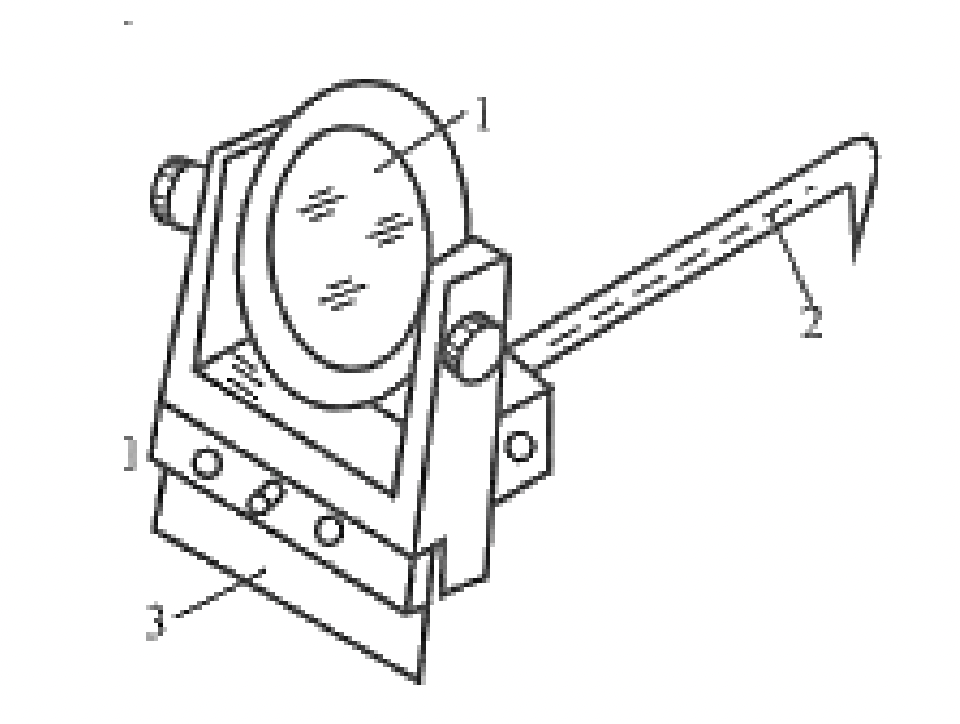
\includegraphics[scale=0.3]{1.png}
    \caption{光杠杆示意图}
    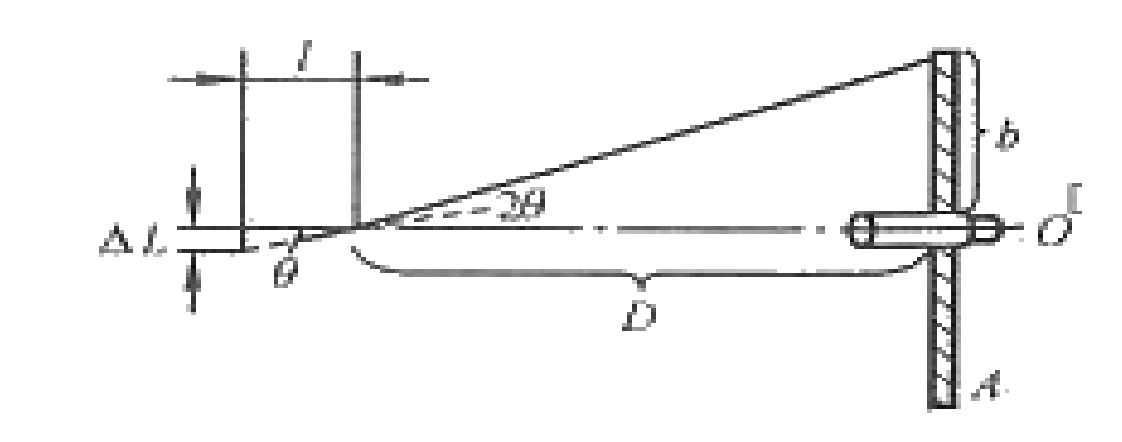
\includegraphics[scale=0.3]{2.png}
    \caption{光路图}
\end{figure}

光杠杆结构如图1所示。杠杆支脚与被测物接触,当被测物发生微小形变时支脚发生移动,平面镜角度随之变化。光路图如图2所示,当角度
变化$\theta$时,入射光角度变化$2\theta$,而这里的$\theta$很小,因此有:
\[\theta \approx \tan \theta =\frac{\Delta L}{l}\]
\[2 \theta \approx \tan 2\theta =\frac{b}{d}\]
结合上面给出的$E$的表达式可以得到:
\[E=\frac{8DLF}{\pi d^2lb}\]
此处使用望远镜观测平面镜成像,望远镜处竖直放置一标尺,用于测量$b$,实验装置如图3.

\begin{figure}[h]
    \centering
    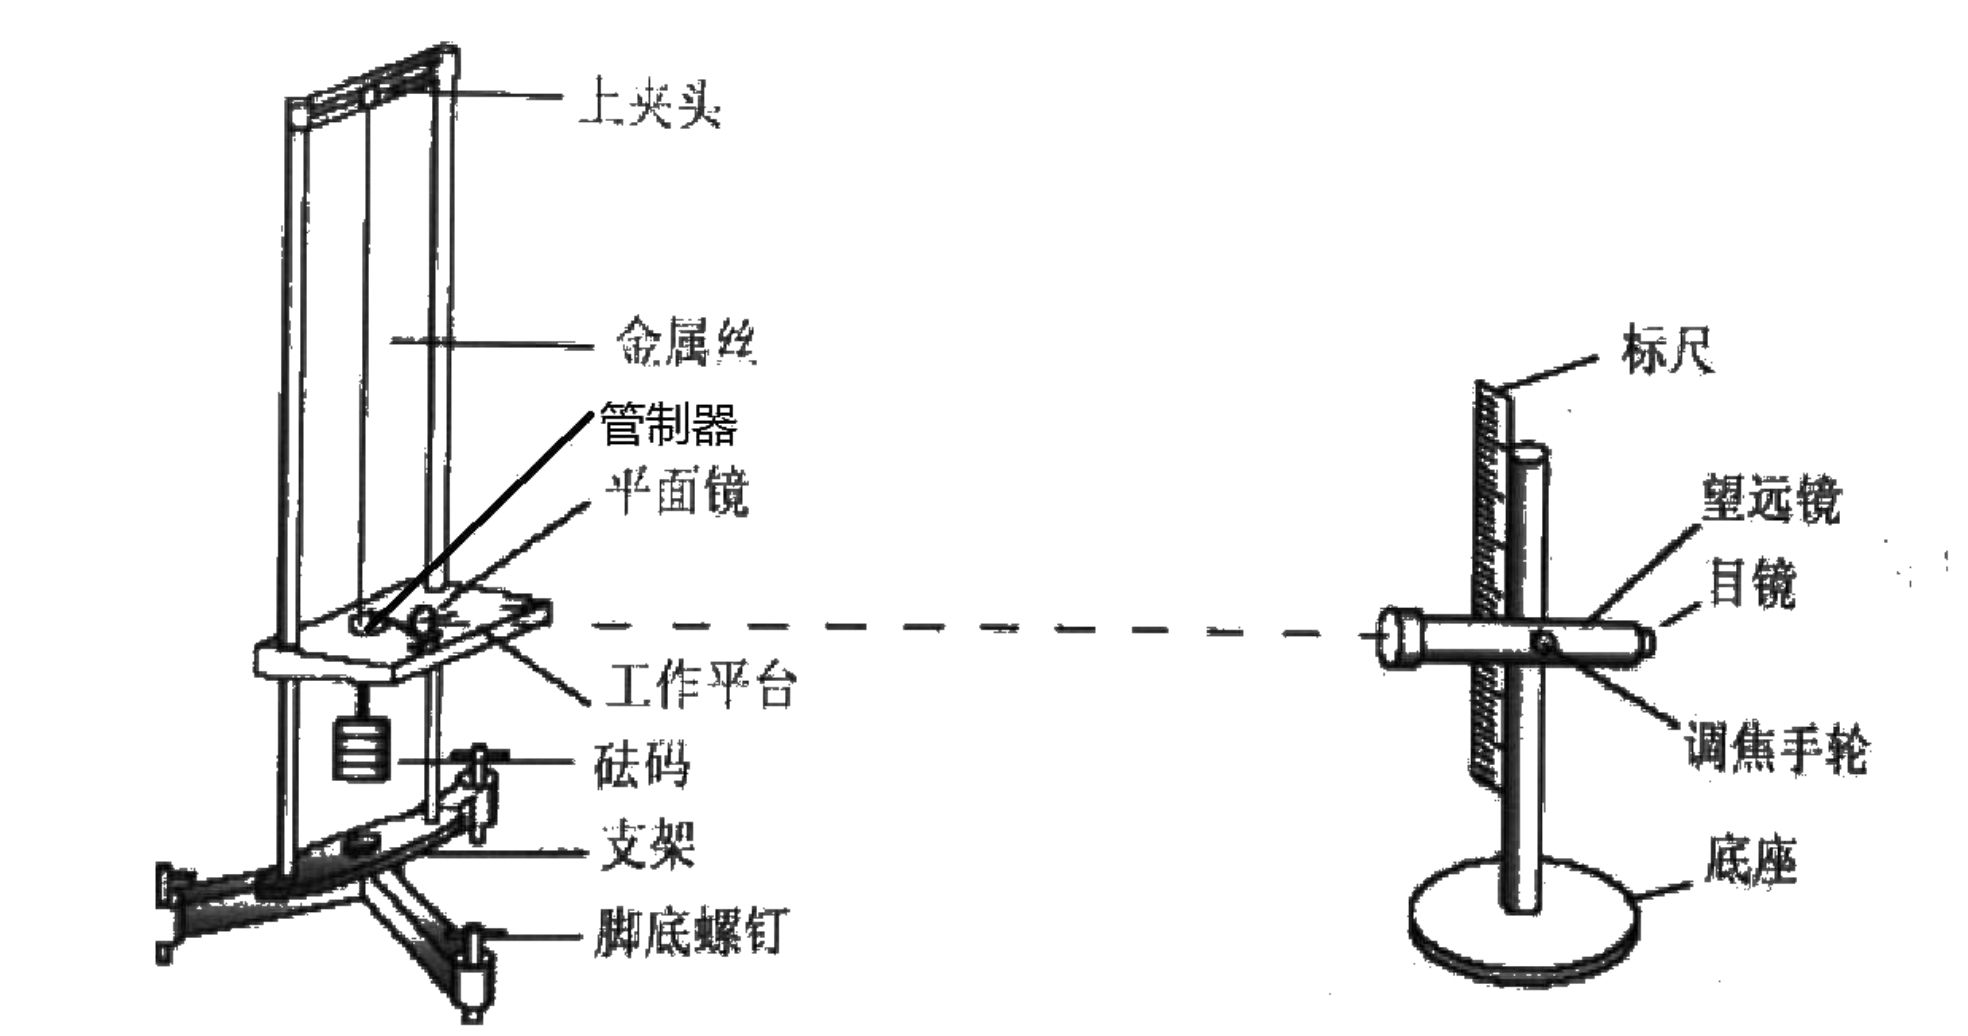
\includegraphics[scale=0.3]{3.png}
    \caption{实验装置示意图}
\end{figure}

因此需要测量的物理量有:钢丝长度$L$,钢丝直径$d$,光杠杆臂长$l$,标尺示数变化$b$,作用力$F$,
标尺到平面镜距离$D$。而从上面的表达式可以看出,$F$与$b$存在线性关系:
\[b=\frac{8DL}{\pi d^2lE}F\]
测出若干组$b$和$F$的值,便能通过线性拟合得到的斜率计算出杨氏模量$E$.
\section{实验数据及计算}
数据如下表
\begin{table}[H]\centering
    \begin{tabular}{ccccc}
        \hline\hline
        测量次数 & $d/ \mathrm{mm}$ & $L/ \mathrm{cm}$ & $D/ \mathrm{cm}$ & $l/ \mathrm{cm}$ \\
        \hline
        1 & 0.295 & 138.33 & 99.78 & 7.15\\
        2 & 0.298 & 138.56 & 99.90 & 7.17\\
        3 & 0.296 & 138.60 & 99.86 & 7.16\\
        4 & 0.296\\
        5 & 0.299\\
        6 & 0.298\\
        \hline\hline
    \end{tabular}
    \caption{$d,L,D,l$的测量值}
\end{table}

此处螺旋测微器零误差为$-0.025\mathrm{mm}$,已对$d$做修正.
\begin{table}[H]\centering
    \begin{tabular}{ccc}
        \hline\hline
        $i$ & $b_i$ & $b_i^{'}$\\
        \hline
        0&0.00&0.02\\
        1&1.30&1.43\\
        2&2.68&2.85\\
        3&4.00&4.20\\
        4&5.45&5.68\\
        5&6.88&6.91\\
        6&8.28&8.29\\
        7&\multicolumn{2}{c}{9.68}\\
        \hline\hline
    \end{tabular}
    \caption{$b_i$及$b_i^{'}$的测量值}
\end{table}
每个砝码重$500\mathrm{g}$,取$g=9.8\mathrm{m/s^2}$,可得到如下结果:
\begin{table}[H]\centering
    \begin{tabular}{ccc}
        \hline\hline
        砝码总质量$m/\mathrm{g}$ & $F/\mathrm{N}$ & $b/\mathrm{cm}$\\
        \hline
        0&0&0.01\\
        500&4.9&1.365\\
        1000&9.8&2.765\\
        1500&14.7&4.1\\
        2000&19.6&5.565\\
        2500&24.5&6.895\\
        3000&29.4&8.285\\
        3500&34.3&9.68\\
        \hline\hline
    \end{tabular}
    \caption{$F$与$b$的值}
\end{table}

\begin{figure}[h]
    \centering
    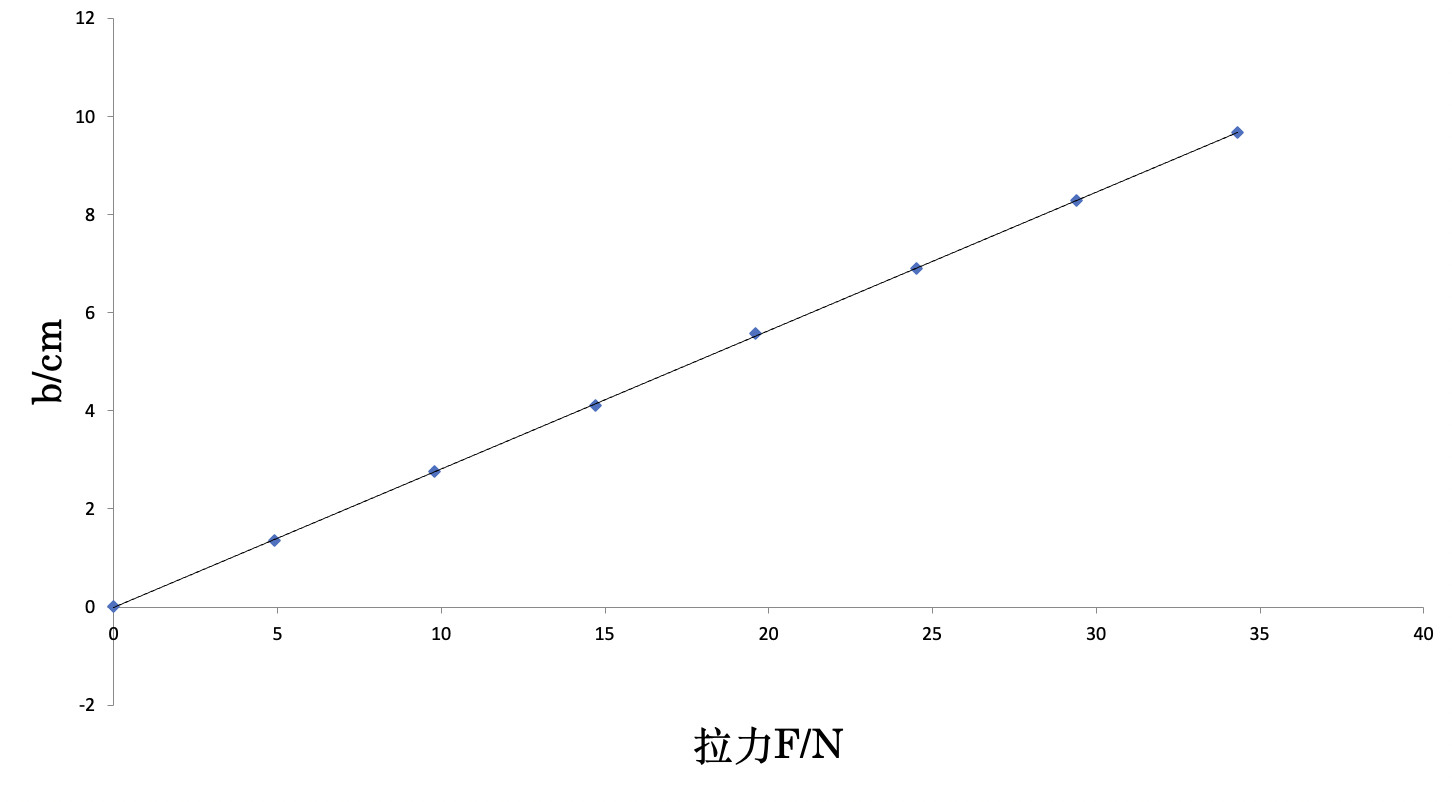
\includegraphics[scale=0.5]{4.png}
    \caption{线性拟合图像}
\end{figure}

图4给出了$b$与$F$的线性拟合图像,拟合得到的斜率与截距为:
\[M=0.28218 \mathrm{cm/N}\]
\[b=-0.00625\mathrm{cm}\]
相关系数
\[r=\frac{\overline{Fb}-\overline{F}\cdot\overline{b}}{\sqrt{\left(\overline{F^2}-\overline{F}^2\right)\left(\overline{b^2}-\overline{b}^2\right)}}=0.99997481\]
斜率的展伸不确定度
\[U_M=t_P\cdot\lvert M\rvert\cdot\sqrt{\frac{\left(\frac{1}{r^2}-1\right)}{n-2}}=0.0020034\,\mathrm{cm/N},P=0.95\]
截距的展伸不确定度
\[U_b=U_M\cdot\sqrt{\overline{F^2}}=0.041065\,\mathrm{cm},P=0.95\]
下面对所测得的其他物理量进行处理
\begin{enumerate}
    \item 钢丝直径$d$
    \[\overline{d}=\frac{1}{n}\sum_{i=1}^{n}d_i=0.297\,\mathrm{mm}\]
    \[\sigma_{d}=\sqrt{\frac{1}{n-1}\sum_{i=1}^n\left(d_i-\overline{d}\right)^2}=0.0015492\,\mathrm{mm}\]
    \[\Delta_{B,d}=\sqrt{\Delta_{app}^2+\Delta_{est}^2}=\sqrt{0.004^2+0.005^2}\,\mathrm{mm}=0.0064031\,\mathrm{mm}\]
    \[U_{d,P}=\sqrt{\left(t_P\frac{\sigma_{d}}{\sqrt{n}}\right)^2+\left(k_P\frac{\Delta_{B,d}}{C}\right)^2}\\=4.4881 \times 10^{-3}\,\mathrm{mm},P=0.95\]
    \item 钢丝长度$L$
    \[\overline{L}=\frac{1}{n}\sum_{i=1}^{n}L_i=138.5\,\mathrm{cm}\]
    \[\sigma_{L}=\sqrt{\frac{1}{n-1}\sum_{i=1}^n\left(L_i-\overline{L}\right)^2}=0.14572\,\mathrm{cm}\]
    \[\Delta_{B,L}=\sqrt{\Delta_{app}^2+\Delta_{est}^2}=0.13\,\mathrm{cm}\]
    \[U_{L,P}=\sqrt{\left(t_P\frac{\sigma_{L}}{\sqrt{n}}\right)^2+\left(k_P\frac{\Delta_{B,L}}{C}\right)^2}=0.37159\,\mathrm{cm},P=0.95\]
    \item 标尺到平面镜距离$D$
    \[\overline{D}=\frac{1}{n}\sum_{i=1}^{n}D_i=99.847\,\mathrm{cm}\]
    \[\sigma_{D}=\sqrt{\frac{1}{n-1}\sum_{i=1}^n\left(D_i-\overline{D}\right)^2}=0.061101\,\mathrm{cm}\]
    \[\Delta_{B,D}=\sqrt{\Delta_{app}^2+\Delta_{est}^2}=0.13\,\mathrm{cm}\]
    \[U_{D,P}=\sqrt{\left(t_P\frac{\sigma_{D}}{\sqrt{n}}\right)^2+\left(k_P\frac{\Delta_{B,D}}{C}\right)^2}=0.17385\,\mathrm{cm},P=0.95\]
    \item 光杠杆臂长$l$
    \[\overline{l}=\frac{1}{n}\sum_{i=1}^{n}l_i=\frac{7.15+7.17+7.16}{3}\,\mathrm{cm}=7.16\,\mathrm{cm}\]
    \[\sigma_{l}=\sqrt{\frac{1}{n-1}\sum_{i=1}^n\left(l_i-\overline{l}\right)^2}\\=0.01\,\mathrm{cm}\]
    \[\Delta_{B,l}=\sqrt{\Delta_{app}^2+\Delta_{est}^2}=0.13\,\mathrm{cm}\]
    \[U_{l,P}=\sqrt{\left(t_P\frac{\sigma_{l}}{估\sqrt{n}}\right)^2+\left(k_P\frac{\Delta_{B,l}}{C}\right)^2}\\=0.088487\,\mathrm{cm},P=0.95\]
\end{enumerate}

\noindent 最终可以得到:
\[E=\frac{8 D L}{\pi d^{2} l M}=1.9759 \times 10^{11}\,\mathrm{Pa}\]
展伸不确定度
\[
\begin{aligned}
    U_{E,P}&=\sqrt{\left(\frac{\partial E}{\partial D}U_{D,P}\right)^2+\left(\frac{\partial E}{\partial L}U_{L,P}\right)^2+\left(\frac{\partial E}{\partial d}U_{d,P}\right)^2+\left(\frac{\partial E}{\partial l}U_{l,P}\right)^2+\left(\frac{\partial E}{\partial M}U_{M,P}\right)^2}\\
    &=6.6325 \times 10^{5}\,\mathrm{N/cm^2},P=0.95
\end{aligned}
\]
杨氏模量的测量值为
\[E=\left(1.98 \pm 0.07\right) \times 10^{7}\,\mathrm{N/cm^2}\]
相对不确定度为$3.535\%$,符合实验要求.
\section{思考题}
\begin{enumerate}
    \item 提高放大率可以使现象更明显,减小因读数产生的误差,但是放大率过大可能会导致超出标尺量程的情况
    \item 长度量的测量与这个长度的大小有关。$d$非常小,只能使用螺旋测微器,如果使用其他仪器会导致相对误差过大
    其余量较大,可以使用钢卷尺。
\end{enumerate}


\bibliography{math}

\end{document}
\iffalse
\begin{figure}[h]
    \centering
    \includegraphics[scale=0.5]{name.png}
    \caption{name}
\end{figure}
\fi
